\section{Rendering Equation(s)}

\subsection{BRDF (Bidirectional Reflectance Distribution Function)}

\textit{Anstatt Diffuse (Gleichmässig) oder Specular (Abnehmend) Reflektion an einem Punkt}

\subsection{Direct \& Indirect Illumination}

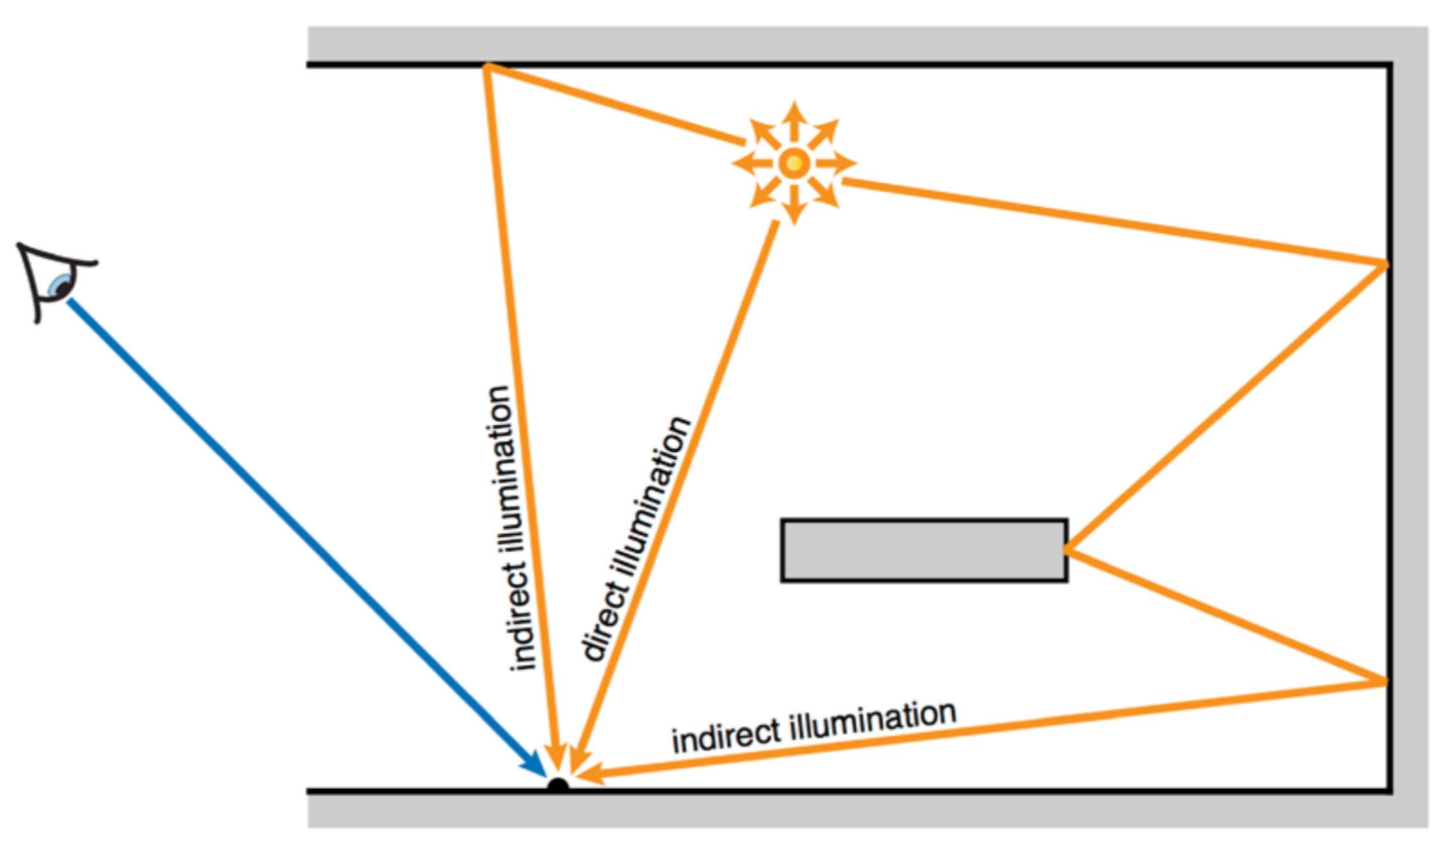
\includegraphics[width=0.4\textwidth]{assets/illumination.png}

\subsection{Radiosity}

\textit{Die beleuchtung der Szene wird vorberechnet ohne die Position der Kamera.
Die Objektoberflächen werden in Patches unterteilt, die Licht reflektieren können.}

\textit{Beleuchtete Fläche als neue Lichtquelle (indirekt)}

\begin{itemize}
    \item Oberflächen unterteilt in "Patches"
    \item "Patch" ist ein Polygon mit konstanter Farbe / Lichtintensität
    \item "Patches" als neue Lichtquelle für andere "Patches"
    \item Das Lichtsystem ist durch lineare Gleichungen zwischen "Patches" modeliert,
        das auflösen dieser ermöglicht die Berechnung der Farbe.
\end{itemize}

Radiositygleichung:\\
$B_i \cdot A_i = E_i \cdot A_i + \rho_i \sum(B_j \cdot A_j \cdot F_{ij})$\\

$B_i$: Radiosity\\
$A_i$: Flächeninhalt des Patches i\\
$E_i$: Emission des Patches i\\
$\rho_i$: Reflektion des Patches i\\
$F_{ij}$: Formfaktor\\

Formfaktorgleichung:\\
$F_{ij} = \frac{1}{A_i}\int_{A_i} \int_{A_j} \frac{\cos \phi \cdot \cos \varphi}{\pi r_{ij}^2} dA_i \cdot dA_j$\\
$A_iF_{ij} = A_jF_{ji}$

\subsection{Radiosity Gleichungen}

\textit{Das Lösen der Gleichungen ist aufwendig. Folgende Methoden gibt es:}

\begin{itemize}
    \item Jacobi Iteration
    \item Gauss Seidel Relaxion
    \item Southwell Iteration
\end{itemize}

\subsection{Progressive Radiosity}

\textit{Berechnung von frühe Darstellung einer approximativer Lösung durch
Patch j auswählen, Radiosity von diesemn Patch j, nächster Patch.}

\subsection{Hirarchical Radiosity}

\textit{Selbe system, doch durch unterschiedliche Patch grösse. Kleine Patches
nahe dem Licht, grosse Patches weiter entfernt.}